

\tikzset{every picture/.style={line width=0.75pt}} %set default line width to 0.75pt        

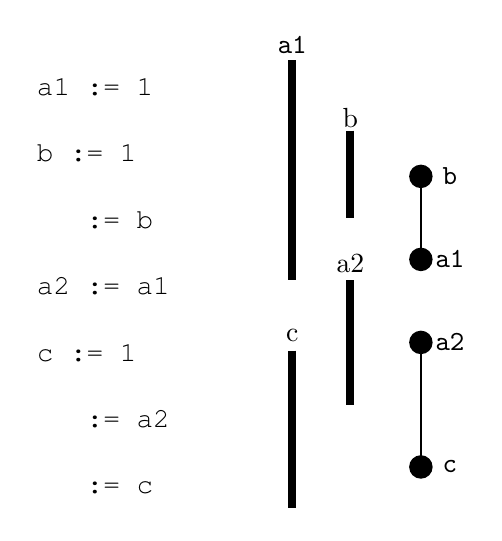
\begin{tikzpicture}[x=0.75pt,y=0.75pt,yscale=-1,xscale=1
                   ,bullet/.style={circle, fill, inner sep=3pt}]
%uncomment if require: 
%\path (0,300); %set diagram left start at 0, and has height of 300

%Shape: Boxed Line [id:dp6151775546096955] 
\draw [line width=1mm] (168, 24) -- (168,130); % a1
\draw [line width=1mm] (196,130) -- (196,190); % a2
\draw [line width=1mm] (196, 58) -- (196,100); % b
\draw [line width=1mm] (168,164) -- (168,240); % c

% Text Node
\draw (77,133) node  [align=left] {
{\fontfamily{pcr}\selectfont a1 := 1}\\\\ 
{\fontfamily{pcr}\selectfont b := 1}\\\\
{\fontfamily{pcr}\selectfont \ \ \ := b}\\\\
{\fontfamily{pcr}\selectfont a2 := a1}\\\\
{\fontfamily{pcr}\selectfont c := 1}\\\\
{\fontfamily{pcr}\selectfont \ \ \ := a2}\\\\
{\fontfamily{pcr}\selectfont \ \ \ := c}};
% Text Node
\draw (168,24.88) node  [align=left] {\tt a1\\};
% Text Node
\draw (196, 60) node  [align=left] {b\\};
\draw (196,130) node  [align=left] {a2\\};
\draw (168,164.86) node  [align=left] {c\\};

\draw (230, 80) node[bullet] {};
\draw (230, 80) node[align=left] {\tt \ \ \ \ b};
\draw (230,120) node[bullet] {};
\draw (230,120) node[align=left] {\tt \ \ \ \ a1};
\draw (230,160) node[bullet] {};
\draw (230,160) node[align=left] {\tt \ \ \ \ a2};
\draw (230,220) node[bullet] {};
\draw (230,220) node[align=left] {\tt \ \ \ \ c};
\draw (230,80)  -- (230,120);
\draw (230,160) -- (230,220); % a
\end{tikzpicture}
